\chapter{GRU应用于模拟数据本构建模研究}
% 3.2表================================================
% 本节仅展示使用常见的三线表
% \begin{table}
% 	\TableBicaption{\label{TDF_para}涵道模型参数}{Parameters of Ducted Fan Model}  % 中英文标题
% 	\centering
% 	\small
% 	\begin{tabularx}{\textwidth}{XXXX}  % 使用 tabularx 环境,均匀分布列宽
% 		\Xhline{1.5pt}
% 		参数符号       & 数值                 & 参数符号  & 数值                 \tabularnewline
% 		\Xhline{0.5pt}  % 表头下方线
% 		$I_x$      & $054593$           & $I_y$ & $0.017045         $ \tabularnewline
% 		$l_1$      & $0.0808\,\text{m}$ & $l_2$ & $0.175\,\text{m}  $ \tabularnewline
% 		$l_4$      & $0.2415\,\text{m}$ & $l_5$ & $0.1085\,\text{m} $ \tabularnewline
% 		$l_\sigma$ & $xdf$              & $df$  & 扫描电镜 \tabularnewline
% 		\Xhline{1.5pt}
% 	\end{tabularx}
% \end{table}
\section{引言}
近年来在深度学习对于流变学的本构建模中研究中,例如Lennon、Mahmoudabadbozchelou等人的研究工作,虽然细节方法各有不同,但是基本在模型选择上都选择普通多层感知机模型(MLP)\cite{lennonScientificMachineLearning2023a,mahmoudabadbozchelouDatadrivenPhysicsinformedConstitutive2021}。MLP是一种经典的前馈人工神经网络,由全连接层堆叠而成,包含输入层、多个隐藏层($\geqslant$1)及输出层,通过非线性激活函数实现复杂函数逼近。当MLP的隐藏层数到达一定值,MLP被视为深度神经网络(DNN)。传统的前馈性质的DNN模型(后简称DNN)具备一定的非线性行为捕捉能力,但是在处理时间序列数据或具有时间依赖性的数据时,其性能可能受到限制。Lennon和Mahmoudabadbozchelou的工作使用DNN模型,很难捕捉到黏弹性材料中的长程应变历史依赖性。本章的研究工作在前人的基础之上尝试使用GRU模型来构建本构建模,期待解决在处理时间序列数据时,DNN模型性能受限的问题。GRU的门控机制允许处理流变学数据,如应力应变数据时,控制历史信息的网络间流动。

本章的研究工作首先采用数值模拟方法构建了经典本构方程的应力应变模拟数据,所涉及的经典本构方程包括Herschel-Bulkley模型、Maxwell模型、Doi-Edwards模型和Giesekus模型。这些模型在流变学领域具有重要的理论和应用价值,能够描述不同类型的流变行为。首先本章研究通过数值模拟方法,生成这些模型的应力应变数据,然后对GRU模型进行了详细的构建,包括模型的结构设计、参数初始化以及训练过程中的优化策略,之后,使用数值模拟生成的应力应变数据GRU模型进行训练,通过调整模型参数和优化算法,使模型能够准确地拟合训练数据。最终本章的研究通过与DNN的训练模型对比,验证了GRU模型在处理时间序列数据时的优势。
\section{实验设计}
\subsection{数值模拟}
本章的数值模拟工作采用Python语言实现,主要依托Numpy、Scipy等高效的数值计算库来完成离散采样和数据处理。
\subsubsection{Herschel-Bulkley模型模拟}
Herschel-Bulkley模型的本构方程如公式\eqref{eq:herschel}所示,其中剪切应力$\sigma$与剪切率$\dot{\gamma}$之间存在函数关系。该模型包含流变参数$K$、流动指数$n$及屈服应力$\sigma_0$。在模拟过程中,本章设置$\sigma_0$为1.0 Pa,$K$为1,而$n$则取值为0.2、0.6、1.0、1.4及1.8。剪切率$\dot{\gamma}$范围设定为[0,100],并以0.01的时间步长进行离散采样。

数据生成后,本章首先采用Matplotlib库绘制出剪切应力$\sigma$与剪切率$\dot{\gamma}$的关系曲线,观察模拟效果,并进行生成效果评估。随后本章采用Numpy库进行数据处理,使用Pandas库将数据存储为Excel文件,便于后续的模型训练。
\subsubsection{Maxwell模型模拟}
Maxwell模型的微分本构方程如公式\eqref{eq:maxwell_model_dt}所示。该模型包含松弛时间$\tau=\eta/\\G$,其中$\eta$表示黏性系数,$G$为剪切模量。本章设置$\eta$为0.1 Pa·s,$G$为1.0 Pa。采用后向欧拉法来离散化微分方程,具体推导如下:

首先将微分离散化,设$d\sigma=\sigma_i - \sigma_{i-1}$,$dt=\Delta t$,$d\gamma=\gamma_i - \gamma_{i-1}$,则原方程可以化简为公式\eqref{eq:maxwell_euler_back_1},
\begin{equation}
  \frac{\sigma_i - \sigma_{i-1}}{\Delta t} + \frac{\sigma_i}{\tau} = G \frac{\gamma_i - \gamma_{i-1}}{\Delta t} \label{eq:maxwell_euler_back_1}
\end{equation}
移项并化简可得公式\eqref{eq:maxwell_euler_back_2}。
\begin{equation}
  \sigma_i = \frac{\sigma_{i-1} + G (\gamma_i - \gamma_{i-1})}{1 + \frac{\Delta t}{\tau}} \label{eq:maxwell_euler_back_2}
\end{equation}
根据公式\eqref{eq:maxwell_euler_back_2},本章首先使用NumPy库生成6个不同应变变化协议的应变数据,时间步为0.01,每个协议模拟2000个数据点,并存为NumPy数组,随后通过迭代法计算单个应变数据对应的应力数据,并存为NumPy数组。之后,本章使用Matplotlib库绘制出剪切应力与剪切应变的关系曲线,观察模拟效果,并进行生成效果评估。最后本章使用Pandas库将数据存储为Excel文件,便于后续的模型训练。
\subsubsection{Doi-Edwards模型模拟}
Doi-Edwards模型的本构方程如公式\eqref{eq:doi_edwards}所示。该方程为积分形式的本构方程,本章首先对该方程进行处理,将取向张量函数$\underline{Q}(t^{\prime},t)$写为球坐标形式,即公式\eqref{eq:doi_edwards_moni_q}。
\begin{align}
   & Q(t^{\prime},t) = \frac{1}{4\pi} \int_{0}^{2\pi} \int_{0}^{\pi} 5 \left( \frac{\underline{\underline{u}}^{\prime} \cdot \underline{\underline{F}}^{-1} \underline{\underline{u}}^{\prime} \cdot \underline{\underline{F}}^{-1}}{|\underline{\underline{u}}^{\prime} \cdot \underline{\underline{F}}^{-1}|^{2}} \right) \sin\theta \, d\theta \, d\phi   \label{eq:doi_edwards_moni_q} \\
   & G(t, t') = \frac{G_0}{\lambda_i} \exp\left( \frac{t' - t}{\lambda_i} \right)   \label{eq:doi_edwards_moni_g}                                                                                                                                                                                                                                                                          \\
   & \sigma(t) = \int_{t_0}^t G(t, t') \cdot Q(\gamma(t')) \, dt' \label{eq:doi_edwards_moni_sigma}
\end{align}

本章模拟的为简单剪切流动,只在xy方向存在应变,因此可以将逆变形梯度张量$\underline{\underline{F}}^{-1}$写为公式\eqref{eq:doi_edwards_f_inverse}的矩阵形式,$\underline{\underline{u}}^{\prime}$为球坐标系下的单位向量。
\begin{equation}
  \underline{\underline{F}}^{-1} = \begin{bmatrix}
    1      & 0 & 0 \\
    \gamma & 1 & 0 \\
    0      & 0 & 1
  \end{bmatrix} \label{eq:doi_edwards_f_inverse}
\end{equation}
公式\eqref{eq:doi_edwards_moni_g}为松弛模量函数,本章使用Numpy库生成7个不同的应变协议的NumPy数组,单个协议时间区间为[0,4$\pi$],总数据点为2000个,生成形式为3*3的张量矩阵,代入公式\eqref{eq:doi_edwards_moni_q}计算$Q$值数组。设置$G_0$为1.0 Pa,$\lambda$为1.0 s,$i=1$,根据公式\eqref{eq:doi_edwards_moni_sigma}计算应变张量,使用的积分工具为Python的scipy.integrate库,生成形式为3*3的张量矩阵,如公式\eqref{eq:sigma_bmatrix}所示。本章提取$
  \sigma_{12}$、$\sigma_{11}$、$\sigma_{22}$分量作为模拟实验数据,与对应的应变分量数据一起通过Pandas库存入Excel文件,便于后续的模型训练。
\begin{equation}
  \sigma = \begin{bmatrix}
    \sigma_{11} & \sigma_{12} & \sigma_{13} \\
    \sigma_{21} & \sigma_{22} & \sigma_{23} \\
    \sigma_{31} & \sigma_{32} & \sigma_{33}
  \end{bmatrix} \label{eq:sigma_bmatrix}
\end{equation}

\subsubsection{Giesekus模型模拟}
Giesekus模型的本构方程如公式\eqref{eq:giesekus}所示,迁移因子$\alpha$用于引入剪切稀化的强度。Giesekus模型模拟的为简单剪切流动,只在xy方向存在应变,应变张量$\boldsymbol{\gamma}$仅在$\gamma_{12}$分量上存在值。
本章首先使用NumPy库生成8个不同应变变化协议的简单剪切流动应变数据,时间区间为[0,24],单个协议的模拟数据点为2000,生成形式为3*3应变张量矩阵,随后设置迁移因子$\alpha$为0.8,其余松弛时间参数($\lambda_1$、$\lambda_2$)为1.0,使用Python的scipy.integrate.solve\_ivp函数(内置方法为Runge-Kutta法)对微分方程组进行求解计算,生成3*3应力张量矩阵,如公式\eqref{eq:sigma_bmatrix}所示。本章提取$\sigma_{12}$、$\sigma_{11}$、$\sigma_{22}$分量作为模拟实验数据,与对应的应变分量数据一起通过Pandas库存入Excel文件,便于后续的模型训练。
\subsection{模型训练}
\subsubsection{数据集划分}
首先本章对模拟生成的数据进行数据集划分,将数据集分为训练集(Train)、验证集(Valid)和测试集(Test),不同模型的具体划分如下:

Herschel-Bulkley模型数据单独划分$n=1.0$的数据为测试集,其余数据按照9:1比例划分为训练集和验证集。

Maxwell模型单独划分4个交变应变协议为训练集和验证集,其中按照9:1比例划分为训练集和验证集。划分1个交变应变协议,1个线性应变协议为测试集。

Doi-Edwards模型单独划分5个交变应变协议为训练集和验证集,其中按照9:1比例划分为训练集和验证集。划分1个交变应变协议,1个线性应变协议为测试集。

Giesekus模型单独划分5个交变应变协议为训练集和验证集,其中按照9:1比例划分为训练集和验证集。划分1个交变应变协议,1个线性应变协议为测试集。
\subsubsection{训练细节}
本章所有模型的训练过程基本一致,首先将数据集划分后,将训练集数据和验证集数据进行归一化,之后转为Torch张量,通过Pytorch框架编写GRU模型代码进行深度学习训练。在训练过程中使用Adam优化算法,使用MSE损失函数,使用
网格搜索算法和随机搜索算法进行超参数优化和选取,训练完成将模型参数保存为.pth文件,以便后续的模型测试。

本章使用GRU和普通DNN(简单MLP)两套模型分别进行训练,训练数据集保持一致。
\subsection{模型测试}
\subsubsection{测试指标细节}
本章的模型训练均为回归问题,所以采用的测试指标为决定系数(R$^2$),如公式\eqref{eq:r2},平均绝对误差(MAE),如公式\eqref{eq:mae}和平均百分比误差(MAPE),如公式\eqref{eq:mape}。
\begin{equation}
  \text{R}^2 = 1 - \frac{\sum_{i=1}^{n} (y_i - \hat{y}_i)^2}{\sum_{i=1}^{n} (y_i - \bar{y})^2} \label{eq:r2}
\end{equation}
\begin{equation}
  \text{MAE} = \frac{1}{n} \sum_{i=1}^{n} |y_i - \hat{y}_i| \label{eq:mae}
\end{equation}
\begin{equation}
  \text{MAPE} = \frac{100\%}{n} \sum_{i=1}^{n} \left| \frac{y_i - \hat{y}_i}{y_i} \right| \label{eq:mape}
\end{equation}
此外,加上训练时间(Training Time)作为训练成本指标。
\subsubsection{不同模型的测试实验划分}
Herschel-Bulkley模型使用训练后保存的模型参数,使用测试集时间进行预测,训练数据与测试数据为不同的流动指数$n$,采用已知流动指数数据预测未知流动指数数据,预测物理量为剪切应力(Stress)。按照上述实验步骤分别使用DNN和GRU两种模型进行测试,绘制两个模型的测试比对曲线。

Maxwell模型训练数据为交变应变数据,其应变关系符合公式\eqref{eq:sin_gamma_protocol},测试数据分为交变应变数据和线性应变数据(公式\eqref{eq:linear_gamma_protocol})。采用已知交变协议数据预测未知交变协议数据,已知交变协议数据预测未知线性协议数据,预测物理量为剪切应力(Stress)。按照上述实验步骤分别使用DNN和GRU两种模型进行测试,绘制两个模型的测试比对曲线。对于GRU模型,设置不同的序列时间步进行训练,探究模型的最佳时间步。
\begin{equation}
  \gamma=\gamma_0cos(\omega t+\phi) \label{eq:sin_gamma_protocol}
\end{equation}
\begin{equation}
  \gamma=\dot{\gamma}t \label{eq:linear_gamma_protocol}
\end{equation}

Doi-Edwards模型和Giesekus模型与Maxwell模型的实验流程一致,采用已知交变协议数据预测未知交变协议数据,已知交变协议数据预测未知线性协议数据,预测物理量为xy方向剪切应力($\sigma_{12}$)和第一法向应力差($\text{N}_1$)。第一法向应力差的公式为$\text{N}_1=\sigma_{11}-\sigma_{12} $,表示模拟流体的弹性行为。按照上述实验步骤分别使用DNN和GRU两种模型进行测试,绘制两个模型的测试比对曲线。对于GRU模型,设置不同的序列时间步进行训练,探究模型的最佳时间步。
\section{结果与讨论}
\subsection{Herschel-Bulkley模型建模}
\subsubsection{数值模拟数据}
本节使用Herschel-Bulkley模型模拟数据,模拟结果如图\ref{herschel_moni}所示。由图\ref{herschel_moni}可以看到,模拟数据中剪切应力(Stress)与剪切速率(Shear Rate)呈现幂函数关系,随着流变指数$n$的增加,曲线的斜率增大,表明流体的非牛顿特性增强。这一现象与Herschel-Bulkley模型的数学形式相符,说明模拟数据符合预期。
\begin{figure}[htbp]
  \centering
  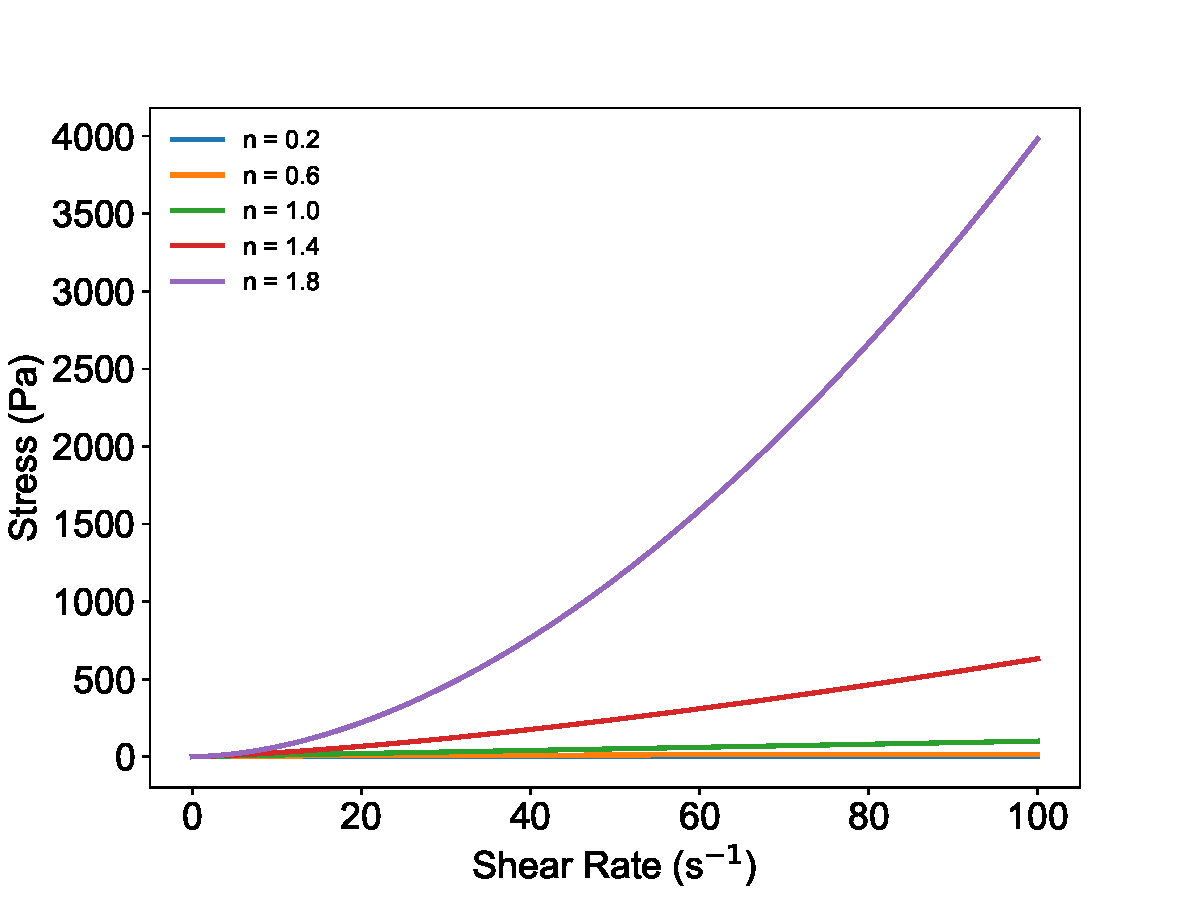
\includegraphics[width=0.8\textwidth]{Fig/herschel_moni.pdf}
  \FigureBicaption{\label{herschel_moni}}{}
\end{figure}
\subsubsection{GRU/DNN模型预测效果对比}
本节分别使用GRU和DNN两种算法对Herschel-Bulkley模型模拟数据进行深度学习建模,之后使用预测模型在测试集上进行验证,测试结果如图\ref{herschel_test}所示。图\ref{herschel_test}(a)为两种算法测试的真实值-预测值曲线,从曲线可以定性看出两种算法的预测值曲线与真实值曲线都非常接近。图\ref{herschel_test}(b)为两种算法测试结果的残差图,可以看出两种算法的残差点离散程度接近,均没有明显趋向性,均呈现无序分布,说明两种算法均可以比较好地捕捉到所有的输入特征。图\ref{herschel_test}(c-f)分别比较了两种算法预测结果的R$^2$,MAE,MAPE指标,从结果中可以看出,两种算法的预测效果都十分良好,R$^2$都接近1,GRU预测结果的R$^2$值略高于DNN,GRU预测结果的MAE和MAPE值都小于DNN,但数值差距不大。GRU算法的平均训练时间为378 s,高于DNN的155 s 一倍以上,这是由于GRU网络的参数量更大,且由于其循环神经网络的特点,只能顺序运算,限制了GPU的并行计算能力,导致训练时间较长。

综合看来GRU和DNN两种算法在Herschel-Bulkley模型模拟数据上的预测表现比较接近,从预测指标的绝对数值看,GRU略优于DNN。这个结果符合预期,因为Herschel-Bulkley模型本质上是模拟了剪切稀化增稠过程,不涉及黏弹性材料的时间依赖性,并且我们模拟的过程中,对于某个特定时间的应力状态也仅仅是当前应变状态的函数。从训练时间的分析看,GRU的训练成本远高于DNN。综合而言对于本构方程类似于Herschel-Bulkley模型的流体,GRU算法虽然在泛化效果上略有优势,但是综合性能上不具备显著优势。
\begin{figure}[htbp]
  \centering
  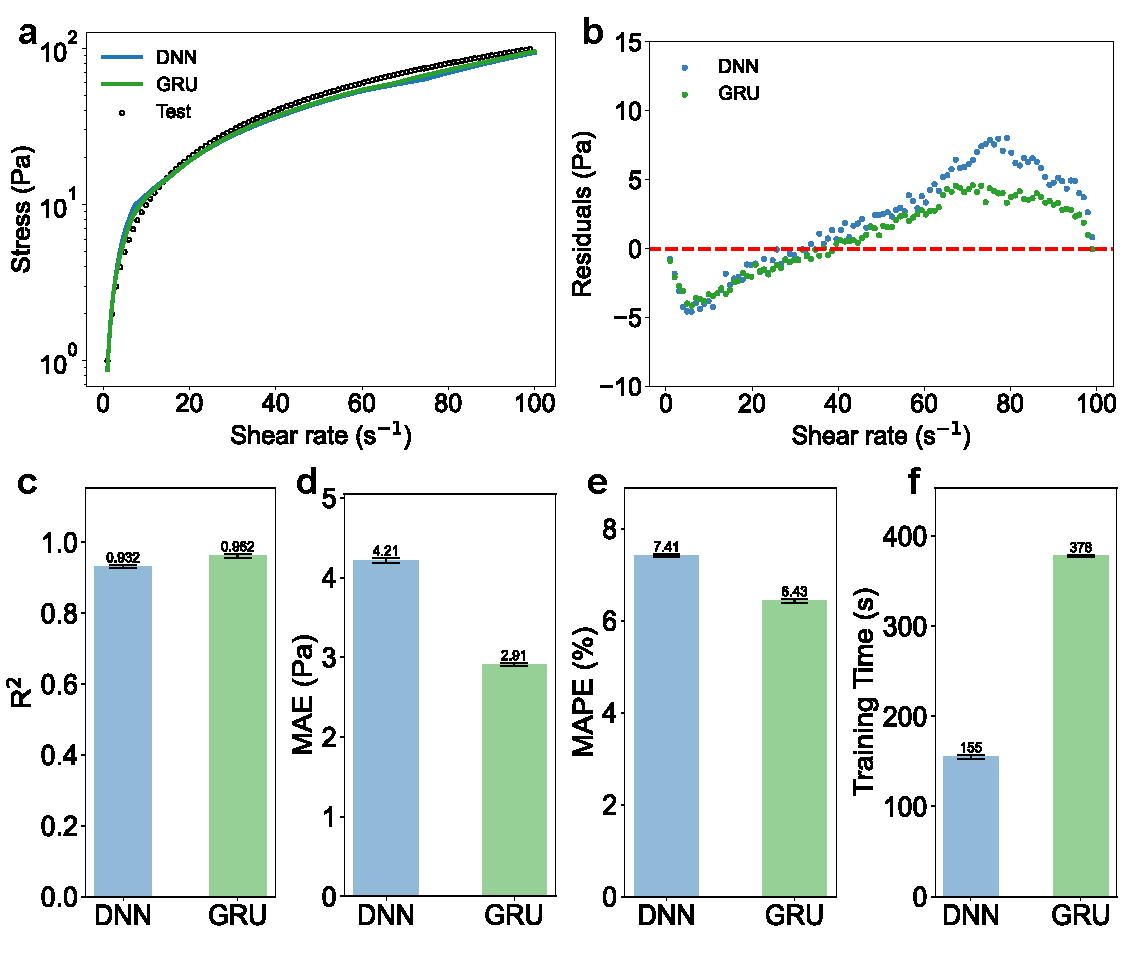
\includegraphics[width=0.8\textwidth]{Fig/Herschel_test.pdf}
  \FigureBicaption{\label{herschel_test}}{}
\end{figure}
\subsection{Maxwell模型建模}
\subsubsection{数值模拟数据}
本节通过后向欧拉法对简单 Maxwell 模型进行了数值模拟,生成了模拟数据,并绘制了应力-应变曲线(Lissajous 曲线),结果如图 \ref{maxwell_moni} 所示。图 \ref{maxwell_moni} 展示了不同应变协议下的模拟结果。对于正弦交变应变,Lissajous 曲线呈现出标准的闭合椭圆形状,这与 Maxwell 模型的理论预期一致,表明模型在周期性应变下的响应具有良好的稳定性和可预测性。对于线性应变,Lissajous 曲线在应变较小时表现出应力的快速增加,随后随着应变的继续增加,应力逐渐趋于一个稳定值,这一现象同样符合 Maxwell 模型的理论预期,反映了材料在持续应变下的应力松弛特性。综合看来,后向欧拉法模拟的数据符合预期,可以用于后续训练。
\begin{figure}[htbp]
  \centering
  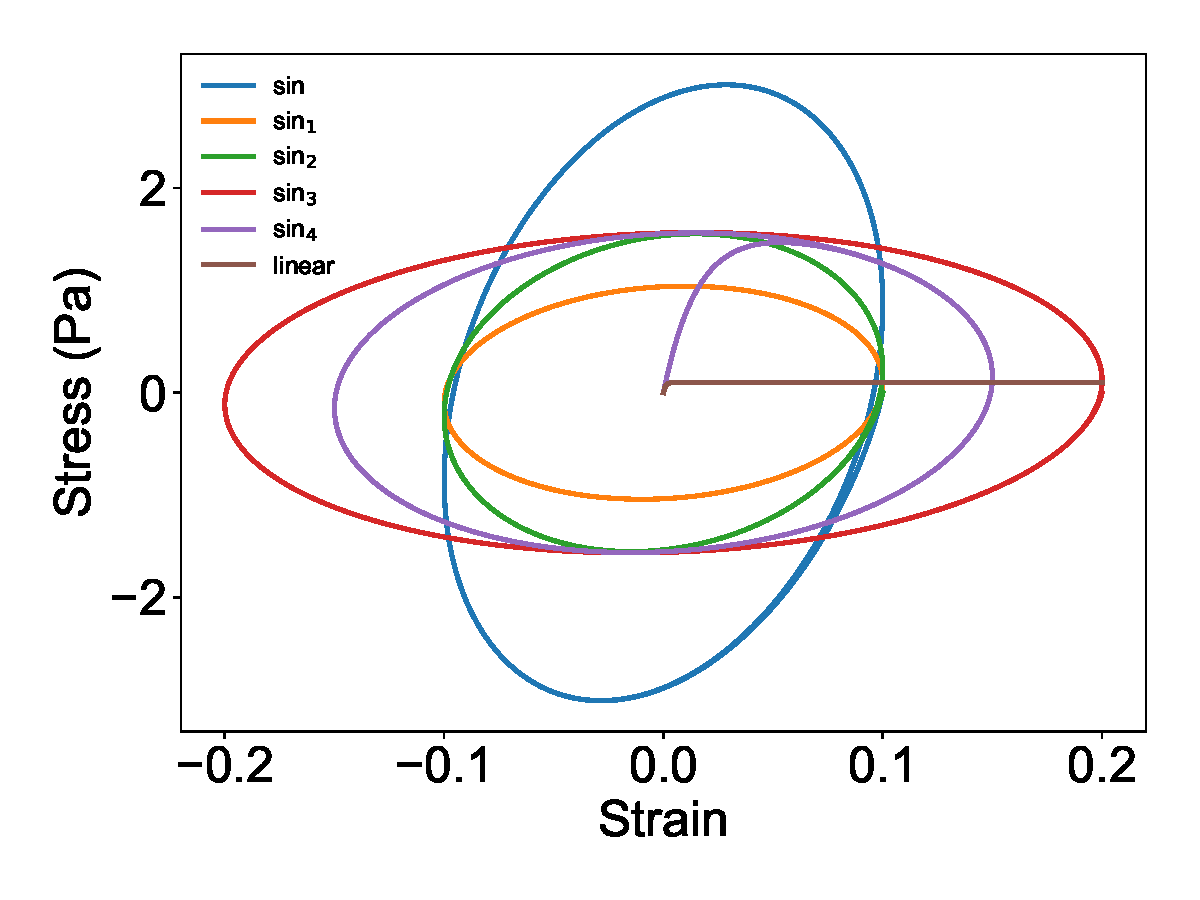
\includegraphics[width=0.8\textwidth]{Fig/maxwell_moni.pdf}
  \FigureBicaption{\label{maxwell_moni}}{}
\end{figure}

\subsubsection{交变协议预测交变协议效果验证}
为了验证GRU算法在时间序列本构方程数据中的预测效果,本节使用交变应变协议生成的数据作为训练集,交变应变协议生成的数据作为测试集。分别使用了GRU和DNN进行训练,并在测试集上进行验证,测试结果如图\ref{maxwell_sin}、图\ref{maxwell_sin_metric}所示。

图\ref{maxwell_sin}(a-b)为两种不同算法预测模型在测试集上的真实值-预测值曲线,
图a为Lissajous曲线,可以看到GRU算法的预测值的Lissajous曲线与真实值曲线十分接近,而DNN算法的预测值的Lissajous曲线与真实的曲线则有明显的周期性偏差,尤其在大应变时,预测值与真实值有较大的偏差。图b为时间-应力曲线,从中可以看到GRU算法的预测值曲线随时间变化较为稳定,贴近真实值曲线,而DNN算法的预测值的曲线明显偏离真实值曲线。

图\ref{maxwell_sin}(c)为两种算法预测模型的测试集残差图,从图中可以看到DNN算法的预测值与真实值残差呈现非常明显的周期性分布,说明DNN未能捕捉到训练数据中的周期性特征,或者说无法泛化到测试集。而GRU的残差图则为无序的近似正态分布,虽然局部存在一定周期性,但是总体正态分布效果明显由于DNN的对应残差,这说明GRU捕捉到了训练数据的较完整的特征,尤其是DNN未能捕捉的周期性特征。综合真实值-预测值曲线和残差图,可以定性分析出GRU的预测效果更为优秀。
\begin{figure}[htbp]
  \centering
  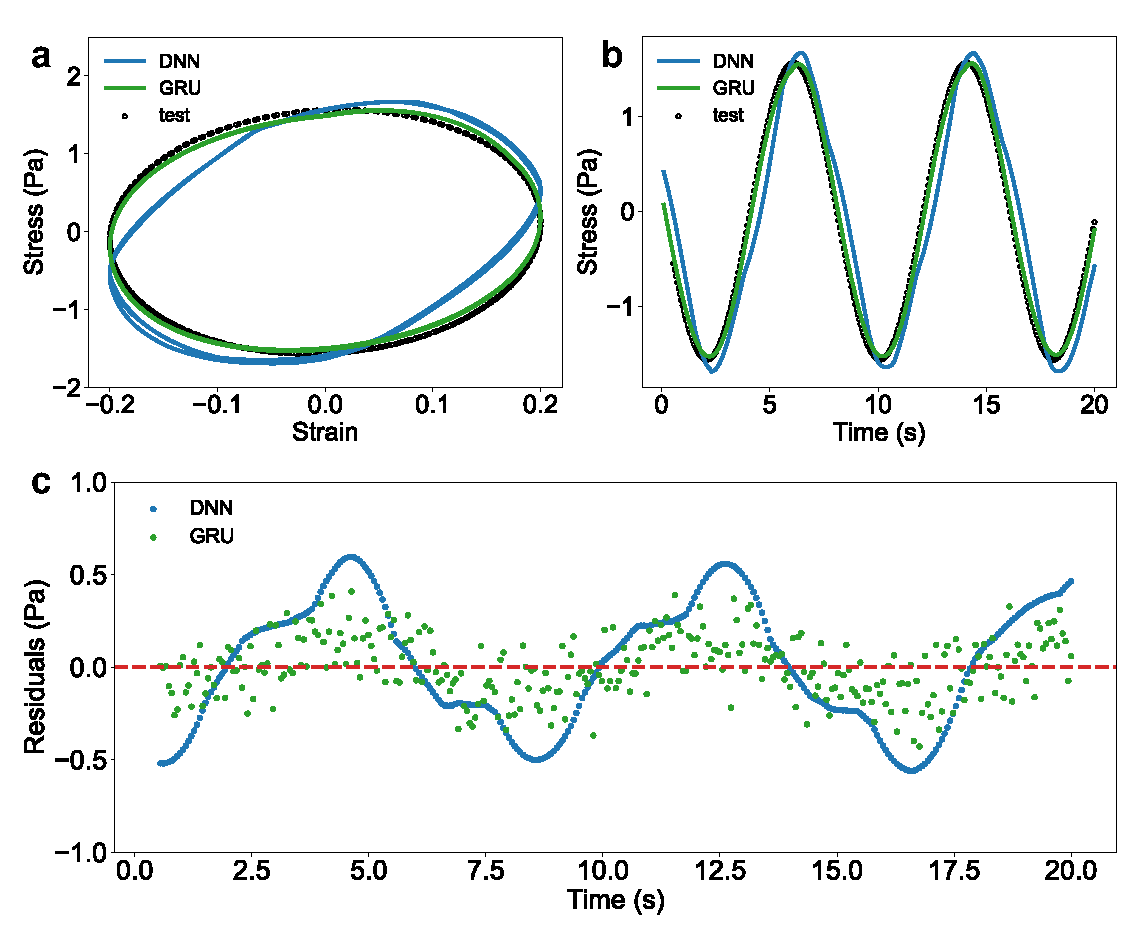
\includegraphics[width=0.8\textwidth]{Fig/Maxwell_sin_.pdf}
  \FigureBicaption{\label{maxwell_sin}}{}
\end{figure}
接下来,本节计算两种算法的测试集预测指标,绘制指标对比图\ref{maxwell_sin_metric}。从图\ref{maxwell_sin_metric
}(a)显示,GRU的R$^2$值为0.986,接近1,说明GRU的预测效果十分优秀,而DNN的R$^2$值为0.904,略低于GRU,但是也高于0.9,属于非常出色的指标。仅从R$^2$指标来看,GRU预测效果优于DNN,但是优势不明显。从图\ref{maxwell_sin_metric}(b-c)看,GRU预测结果的MAE值为0.019,仅为DNN预测结果的MAE值的一半,GRU预测结果的MAPE值为3.09,仅为DNN预测结果的MAPE值14.95的五分之一左右。这定量说明GRU的预测结果误差远小于DNN的预测结果误差,GRU在此项任务上预测泛化效果更好。当然,由于GRU的模型特性,其训练时间如图\ref{maxwell_sin_metric}(d)所示,要高于DNN。
\begin{figure}[htbp]
  \centering
  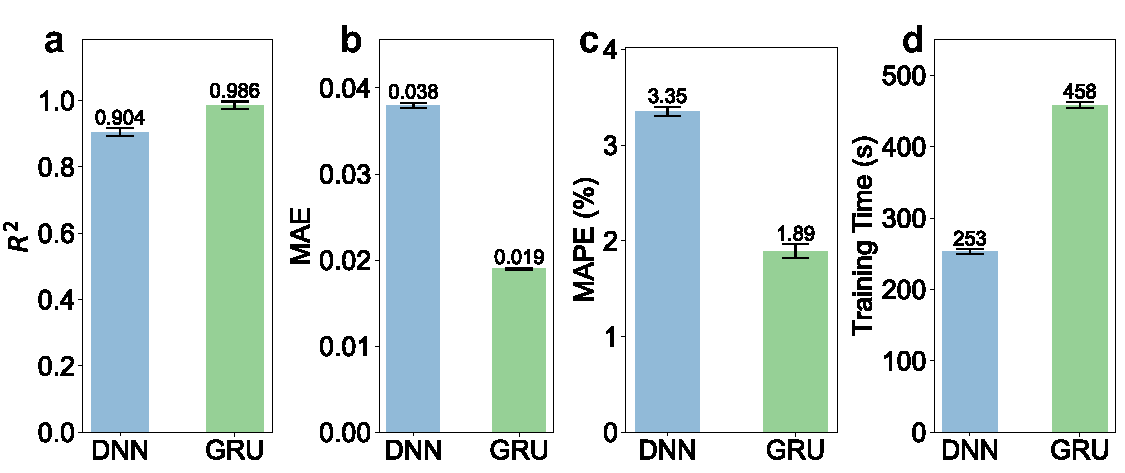
\includegraphics[width=0.8\textwidth]{Fig/Maxwell_sin_metric.pdf}
  \FigureBicaption{\label{maxwell_sin_metric}}{}
\end{figure}
综合各项分析数据来看,当训练数据和测试数据为同类型应变变化过程(都为交变应变)时,GRU算法可以更好的学习到Maxwell模型数据的内在特征,包括周期性响应,黏弹性,时间依赖性响应。从定性与定量分析结果看,GRU算法的预测泛化效果在此项任务上明显优于DNN,在计算资源足够时,GRU算法相比DNN性能更佳。


\subsubsection{交变协议预测线性协议效果验证}
为了验证GRU算法在不同形式的应变历史下的泛化预测效果,本节使用交变应变协议生成的数据作为训练集,线性应变协议生成的数据作为测试集。分别使用了GRU和DNN进行训练,并在测试集上进行验证,测试结果如图\ref{maxwell_linear}、图\ref{maxwell_linear_metric}所示。

图\ref{maxwell_sin}(a-b)为两种不同算法预测模型在测试集上的真实值-预测值曲线,
图a为Lissajous曲线,可以看到GRU算法的预测值的Lissajous曲线与真实值曲线十分接近,而DNN算法的预测值的Lissajous曲线与真实的曲线则有明显的周期性偏差,尤其在大应变时,预测值与真实值有较大的偏差。图b为时间-应力曲线,从中可以看到GRU算法的预测值曲线随时间变化较为稳定,贴近真实值曲线,而DNN算法的预测值的曲线明显偏离真实值曲线。

图\ref{maxwell_sin}(c)为两种算法预测模型的测试集残差图,从图中可以看到DNN算法的预测值与真实值残差呈现非常明显的周期性分布,说明DNN未能捕捉到训练数据中的周期性特征,或者说无法泛化到测试集。而GRU的残差图则为无序的近似正态分布,虽然局部存在一定周期性,但是总体正态分布效果明显由于DNN的对应残差,这说明GRU捕捉到了训练数据的较完整的特征,尤其是DNN未能捕捉的周期性特征。综合真实值-预测值曲线和残差图,可以定性分析出GRU的预测效果更为优秀。
\begin{figure}[htbp]
  \centering
  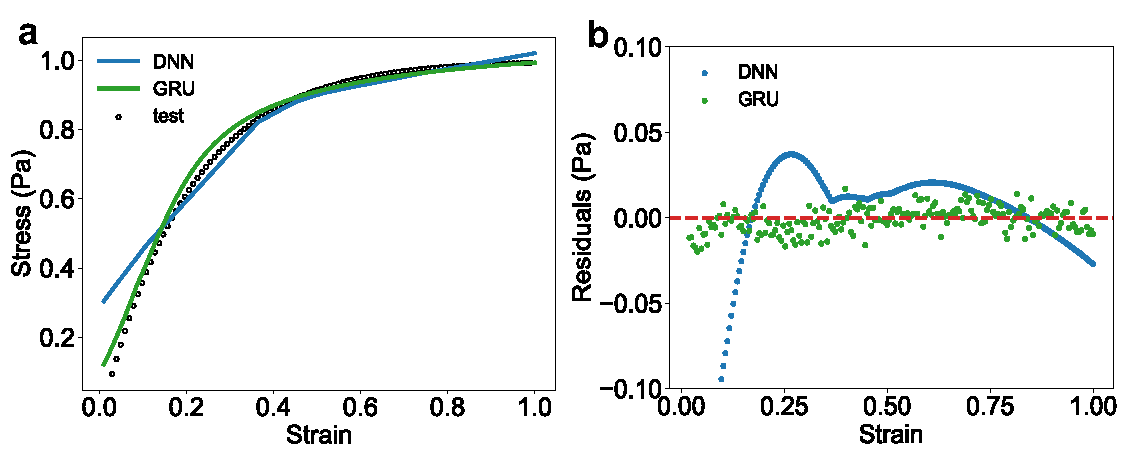
\includegraphics[width=0.8\textwidth]{Fig/maxwell_linear_test.pdf}
  \FigureBicaption{\label{maxwell_linear}}{}
\end{figure}
接下来,本节计算两种算法的测试集预测指标,绘制指标对比图\ref{maxwell_sin_metric}。从图\ref{maxwell_sin_metric
}(a)显示,GRU的R$^2$值为0.986,接近1,说明GRU的预测效果十分优秀,而DNN的R$^2$值为0.904,略低于GRU,但是也高于0.9,属于非常出色的指标。仅从R$^2$指标来看,GRU预测效果优于DNN,但是优势不明显。从图\ref{maxwell_sin_metric}(b-c)看,GRU预测结果的MAE值为0.019,仅为DNN预测结果的MAE值的一半,GRU预测结果的MAPE值为3.09,仅为DNN预测结果的MAPE值14.95的五分之一左右。这定量说明GRU的预测结果误差远小于DNN的预测结果误差,GRU在此项任务上预测泛化效果更好。当然,由于GRU的模型特性,其训练时间如图\ref{maxwell_sin_metric}(d)所示,要高于DNN。
\begin{figure}[htbp]
  \centering
  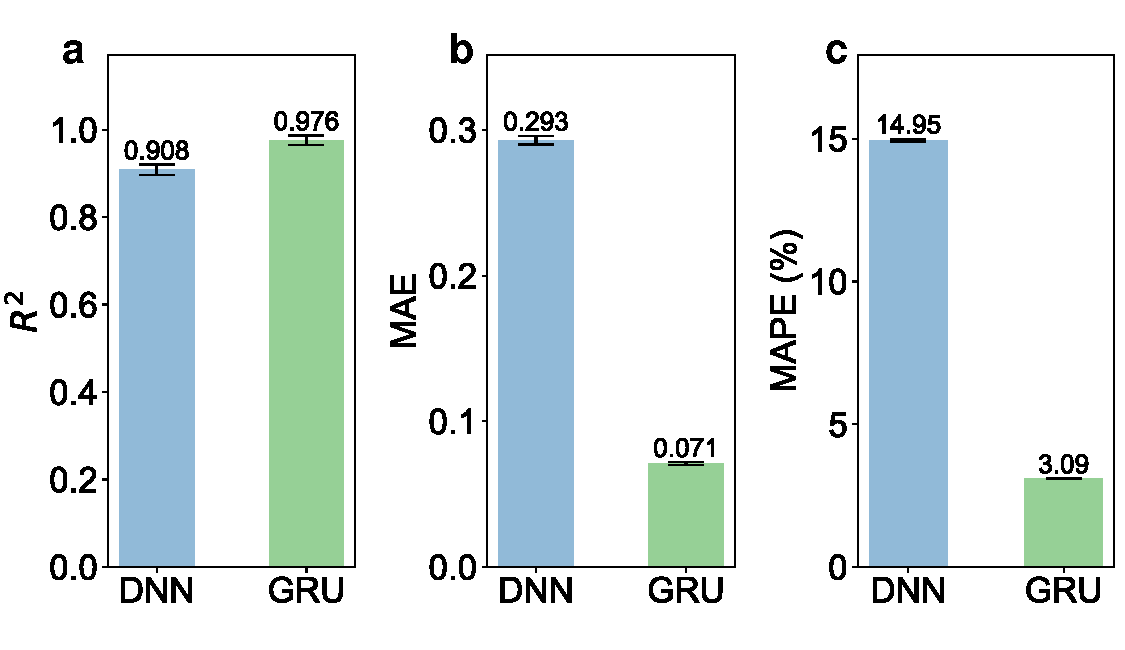
\includegraphics[width=0.8\textwidth]{Fig/maxwell_linear_metric.pdf}
  \FigureBicaption{\label{maxwell_linear_metric}}{}
\end{figure}
综合各项分析数据来看,当训练数据和测试数据为同类型应变变化过程(都为交变应变)时,GRU算法可以更好的学习到Maxwell模型数据的内在特征,包括周期性响应,黏弹性,时间依赖性响应。从定性与定量分析结果看,GRU算法的预测泛化效果在此项任务上明显优于DNN,在计算资源足够时,GRU算法相比DNN性能更佳。

\subsubsection{不同时间步的预测效果对比}

\begin{figure}[htbp]
  \centering
  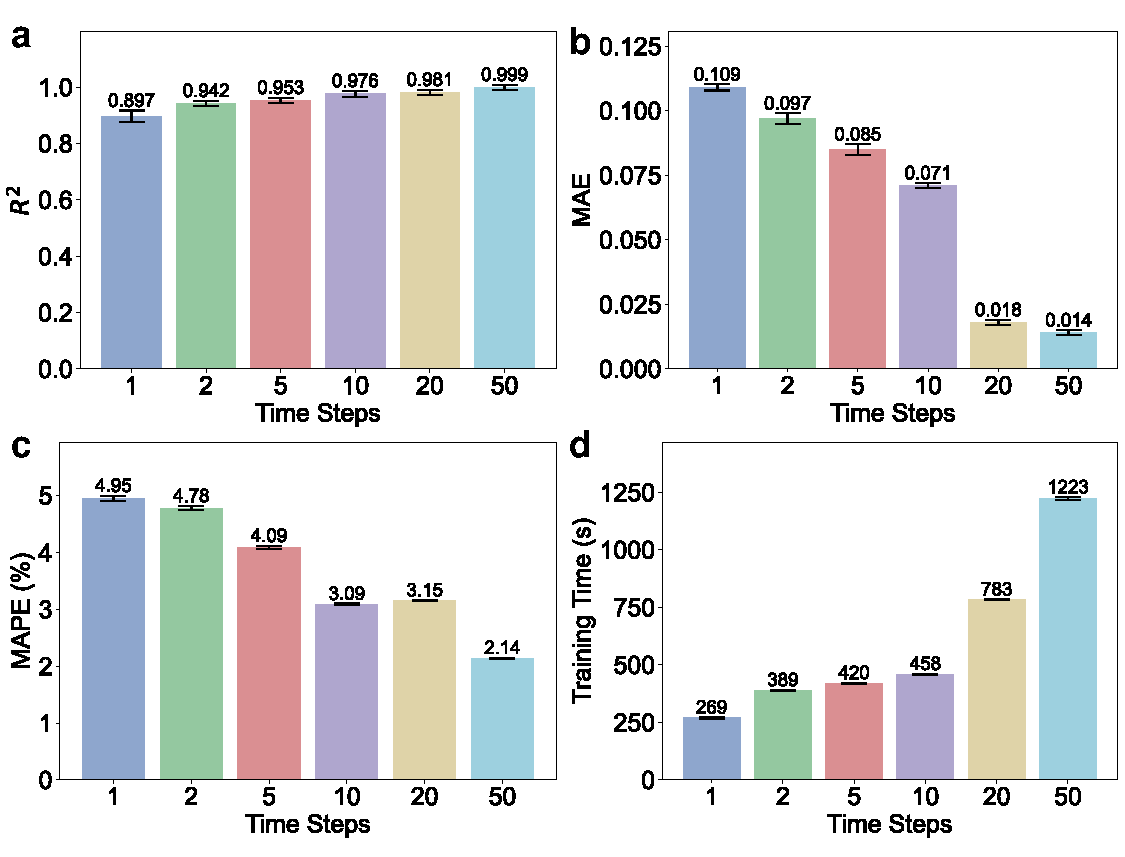
\includegraphics[width=0.8\textwidth]{Fig/Maxwell_timesteps_metrics.pdf}
  \FigureBicaption{\label{maxwell_timesteps_metrics}}{}
\end{figure}

\subsection{Doi-Edwards模型建模}
\subsubsection{数值模拟数据}
sff
\subsubsection{交变协议预测交变协议效果验证}
\subsubsection{交变协议预测线性协议效果验证}
\subsubsection{不同时间步的预测效果对比}
\subsection{Giesekus模型建模}
\subsubsection{数值模拟数据}
sff
\subsubsection{交变协议预测交变协议效果验证}
\subsubsection{交变协议预测线性协议效果验证}
\subsubsection{不同时间步的预测效果对比}
\section{本章小结}













